\chapter{Fazit}
\label{chap:Fazit}
Die Arbeit schließt mit einer Zusammenfassung der Inhalte ab, auf welche eine kritische Auseinandersetzung mit verschiedenen Ergebnissen der Abschlussarbeit folgt und durch einen ausführlichen Blick auf mögliche Erweiterungen, weiterer Forschungsbedarf und weitere geleistete Arbeiten komplettiert wird.
 
	\section{Zusammenfassung}
	\label{sec:Zusammenfassung}
	Ziel dieser Arbeit war es ein Verfahren zu entwickeln um den Einsatz von annotierten Daten zu reduzieren, hierzu wurden die theoretischen Hintergründe, das Umfeld der Problemstellung und die Datensätze vorgestellt. Der Hauptteil der Arbeit beschäftigt sich mit aufeinander aufbauenden Ansätzen des Transferlernens. Im ersten Schritt wurde gezeigt, dass ein Ansatz, ausgehend von einer nicht fokussierten Repräsentation fehlschlägt. Darauf folgend wurde ein \acl{mtl}-Ansatz zum gleichzeitigen Fokussieren und Lösen einer Regressionsaufgabe vorgestellt und evaluiert. Insbesondere die gefundene Repräsentation hat dabei deutlich die aktuelle Domäne widergespiegelt. Darauf aufbauend wurde ein Ansatz des modellbasierten Transferlernens vorgestellt. Die Ergebnisse erreichen eine ähnliche Leistung wie das Basislinienmodell. Zur \ac{hpo} der Aufgabengewichtung wurde eine \ac{automl}-Erweiterung eingesetzt. Dabei hat sich gezeigt, dass der Hyperparameter einen deutlichen Einfluss auf das Ergebnis hat und die automatische Suche hilfreich ist. Abschließend wurde gezeigt, dass die Transfer-Lösung insbesondere für geringe Datenmengen gute Ergebnisse liefern kann. Begleitend zu der Vorstellung der Ansätze wurde jeweils eine Python-Implementierung des Ansatzes vorgestellt. 
	
	\section{Kritische Reflexion}
	\label{sec:KritischeReflexion}
	Auf Grund des Umfangs der vorliegenden Arbeit wurde das Module \ac{autottae} nur oberflächlich angerissen. Bei zukünftigen Arbeiten empfiehlt es sich, eine Optimierung mit deutlich mehr Iterationen und weiteren zu optimierenden Hyperparametern durchzuführen.
	
	Auf Grund der Einfachheit (vier Ausgangsneuronen) wurde für die Aufgabe 'Rahmen um Greifer' eine Regression eingesetzt. In der Regel werden für Objekterkennungsaufgaben andere Techniken wie z.B. der bereits erwähnte \ac{ssd}-Ansatz eingesetzt. Durch eine explizite Lokalisierung und Klassifizierung werden oft bessere Ergebnisse erzielt.
	
	Die bisherigen Versuche wurden alle in derselben Domäne, mit  Bilder und dem Greifer durchgeführt. Die gewählten Ansätze wurden für diese Umgebung gewählt. Die Aussagekraft auf andere Domänen oder Umgebungen mit weniger stark ausgeprägten Merkmalen, wie ein Greifer, ist schwach und sollte in weiteren Versuchen untersucht werden.    
							
	\section{Ausblick und weitere Arbeiten}
	\label{sec:AusblickWeitereArbeiten}
	In diesem letzten Unterkapitel werden weitere (vorläufige) Ergebnisse dargestellt und ein Blick auf mögliche Erweiterungen geworfen.

	\subsection{Transfer auf Greiferdatensatz}
	\label{subsec:TransferGreiferDatensatz}
 	Die Annotationskosten sind je nach Art von Annotation und Aufwand unterschiedlich. Eine einfache Zuordnung eines Bildes zu einer von zwei Klassen liegt dabei im einstelligen Cent-Bereich. Die Markierung eines Objektes in einem Bild mittels Rahmen verursacht Kosten im zweistelligen Cent-Bereich und die Markierung von Winkeln in einem Bild kann mehr als einen Euro kosten. In Kapitel \ref{sec:TransferDatenmenge} und \ref{subsec:TransferLogs} wurde gezeigt, dass der Transfer für die Aufgabe 'Greifer beladen?' funktioniert und insbesondere bei wenigen Daten stark ist. Sofern ein Transfer von der Aufgabe 'Greifer beladen?' zu der Aufgabe 'Rahmen um Greifer' möglich ist, sind deutliche Kosteneinsparungen zu erreichen, da hier die Annotationen kostenintensiver sind. 
 	
 	Im ersten Versuch ist der Transfer auf dem Greiferdatensatz fehlgeschlagen, durch weitere Arbeiten an dem Problem konnte eine Verbesserung erzielt werden. Zu den weiteren Arbeiten zählen das Entfernen von Bildern, bei denen der Greifer über den Rand des Bildes hinausgeht. Diese Bildern können durch eine Modifikation der Kameraposition am Kran nicht mehr vorkommen. Weitere Verbesserungen konnten durch Regularsierungstechniken erzielt werden. Im Anhang \ref{appendix:TTAEGreifer } ist die aktuelle Modellzusammenfassung zu finden. \\
 	In Abbildung \ref{img:TTGrappleIoU} sind die Ergebnisse der Aufgabe 'Rahmen um Greifer' dargestellt. Bei einem Schwellenwert von 0.5 wird eine Leistung von 96\% erreicht und bei einem Schwellenwert 0.8 eine Leistung von 55\%. Bei genauerer Betrachtung der Vorhersagen fällt auf, dass der Greifer gefunden wird, die genauen Abmessungen aber nicht korrekt sind. Dieses Verhalten ist auch in Abbildung \ref{img:TTGrappleLabelVsPred} zu sehen. In dieser Art von Abbildungen werden die Vorhersagen gegen die Beschriftungen aufgetragen. Bei einer perfekten Vorhersage befinden sich alle Datenpunkte auf der Diagonale. Sowohl in der Darstellung der Rahmenhöhe als auch der Rahmenbreite ist zu sehen, dass die Vorhersage zur Beschriftung passt, aber sich noch verbessern kann. In Abbildung \ref{img:TTGrappleEinbettungVorhersage} sind die für den Schwellenwert 0.8 falsch vorhergesagten Datenpunkte in der Einbettung lila eingefärbt. Die falschen Vorhersagen verteilen sich über alle Datenpunkte. Mit Blick auf die Einfärbung der x und y Position des Greifers \ref{img:TTGrappleEmb}, zeigt sich in den Einbettungen die Position des Greifers im Bild. Widerspiegeln zu den Vorhersageergebnissen ist in der Einbettung die genaue Ausprägung des Greifers schwach repräsentiert.
 	\begin{figure}[h]
 		\centering
 
 		\begin{subfigure}[c]{0.49\textwidth}			
 			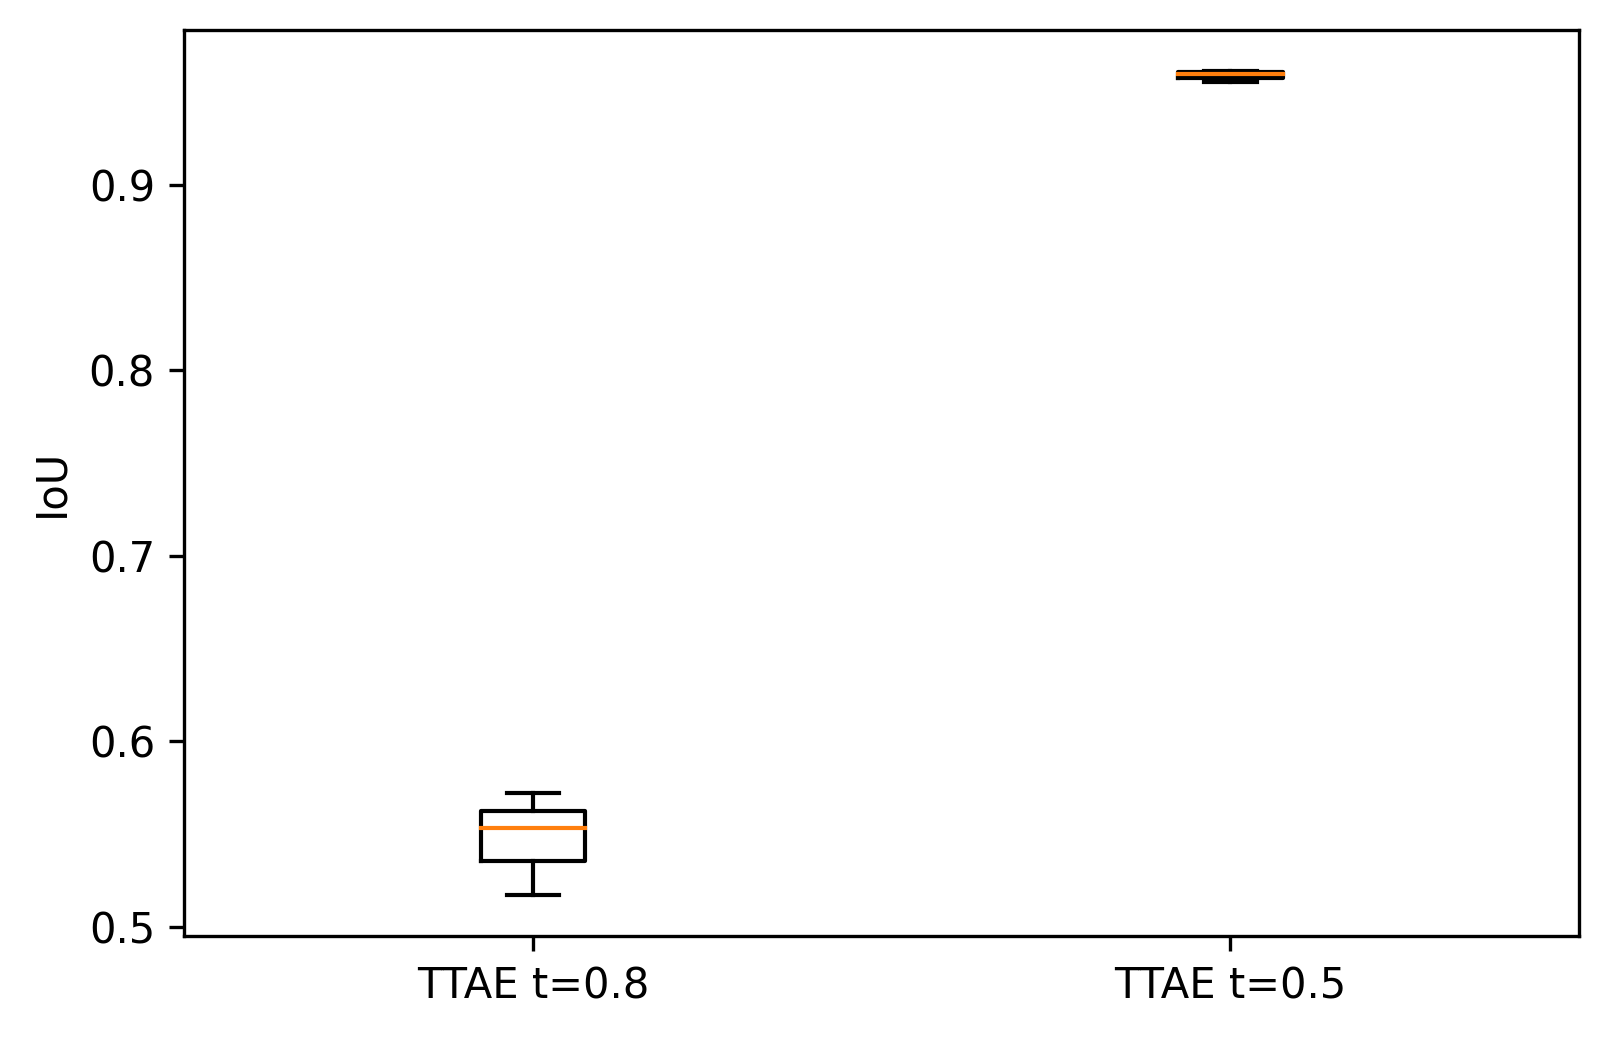
\includegraphics[width=1\textwidth]{bilder/FazitUndAusblick/Grapple_TTAE_Res/IoU_TTAE_0805.png}
 			\subcaption{Ergebnisse bei drei Durchläufen und einem Schwellenwert von 0.8 und 0.5}			
 		\end{subfigure}
 		\begin{subfigure}[c]{0.49\textwidth}			
 			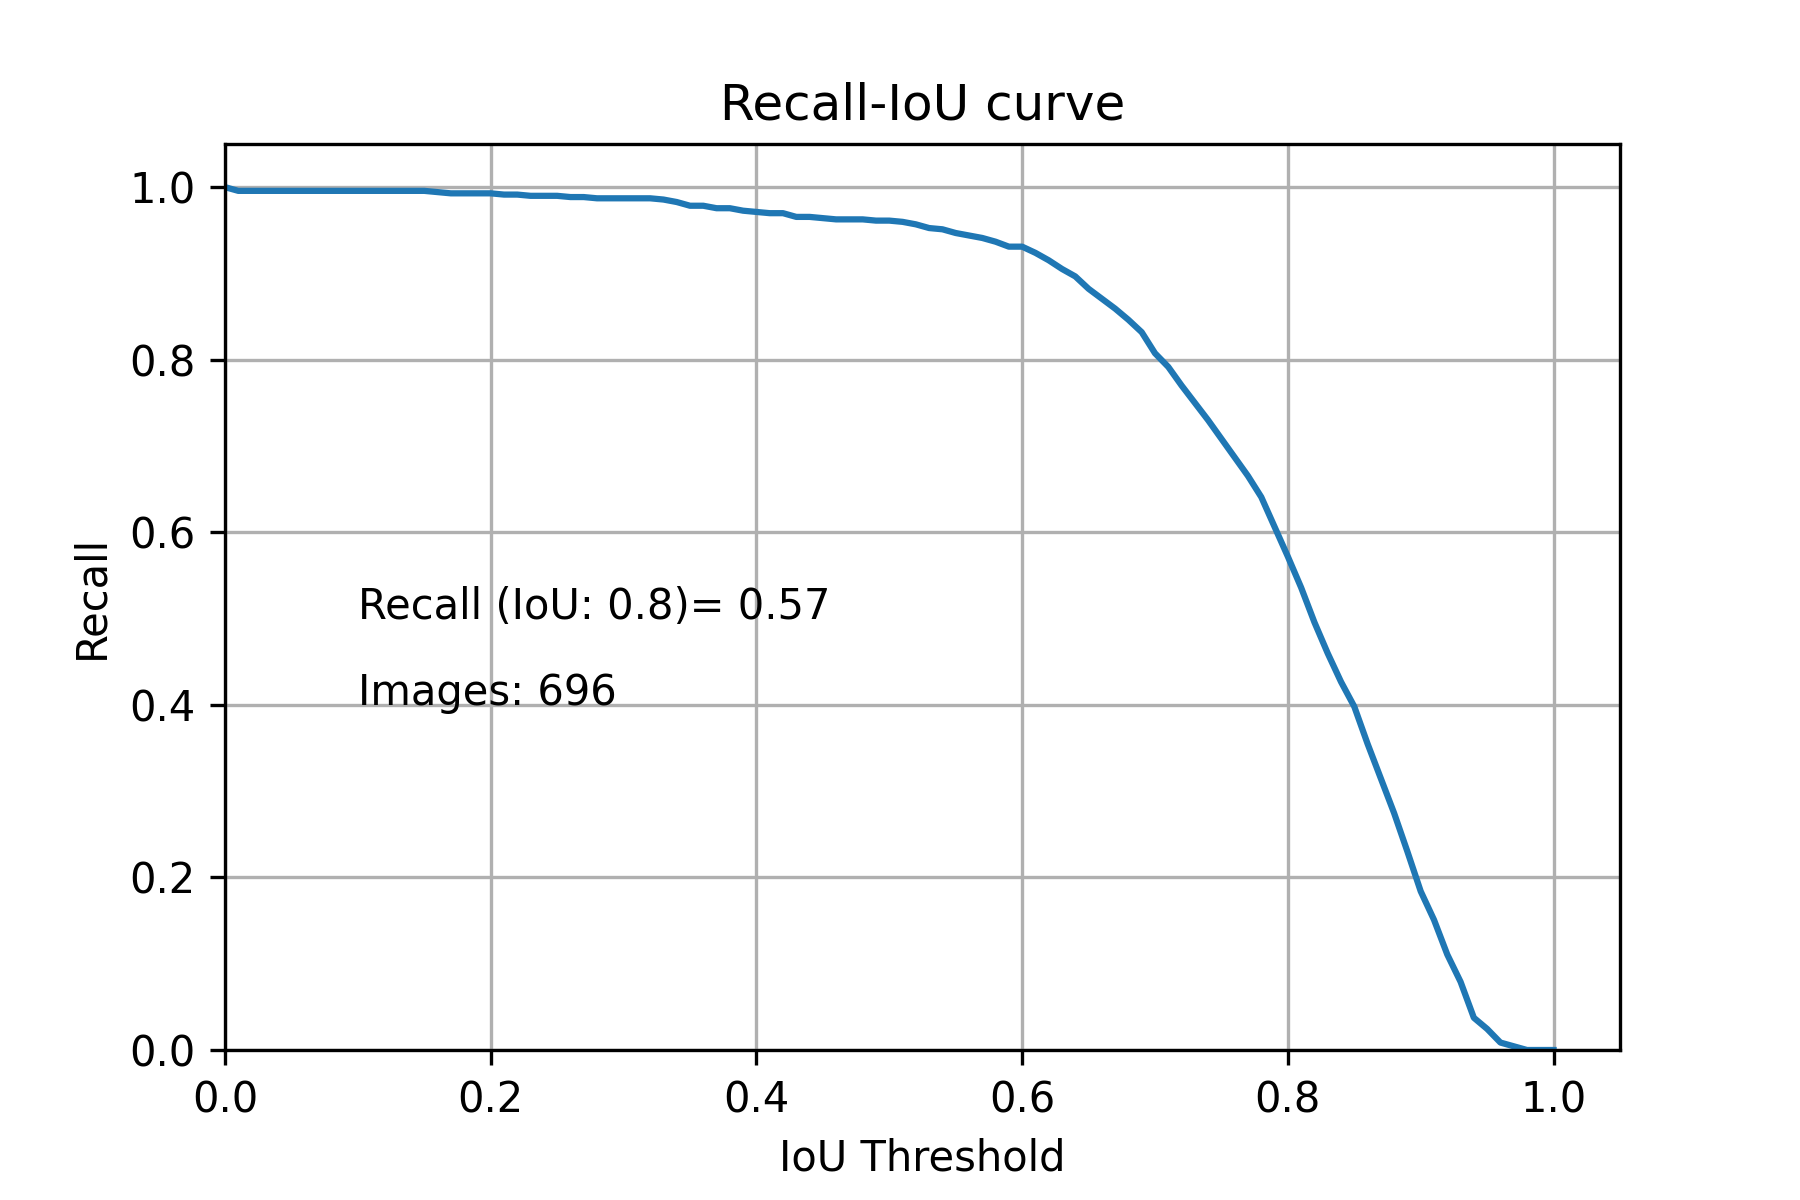
\includegraphics[width=1\textwidth]{bilder/FazitUndAusblick/Grapple_TTAE_Res/Recall_IoU_TTAE.png}
 			\subcaption{IoU-Recall-Curve}			
 		\end{subfigure}
 		\caption{IoU TTAE Greifer}
 		\label{img:TTGrappleIoU}
 	\end{figure}
 
 	 	\begin{figure}[h]
 		\centering
 		\begin{subfigure}[c]{0.49\textwidth}			
 			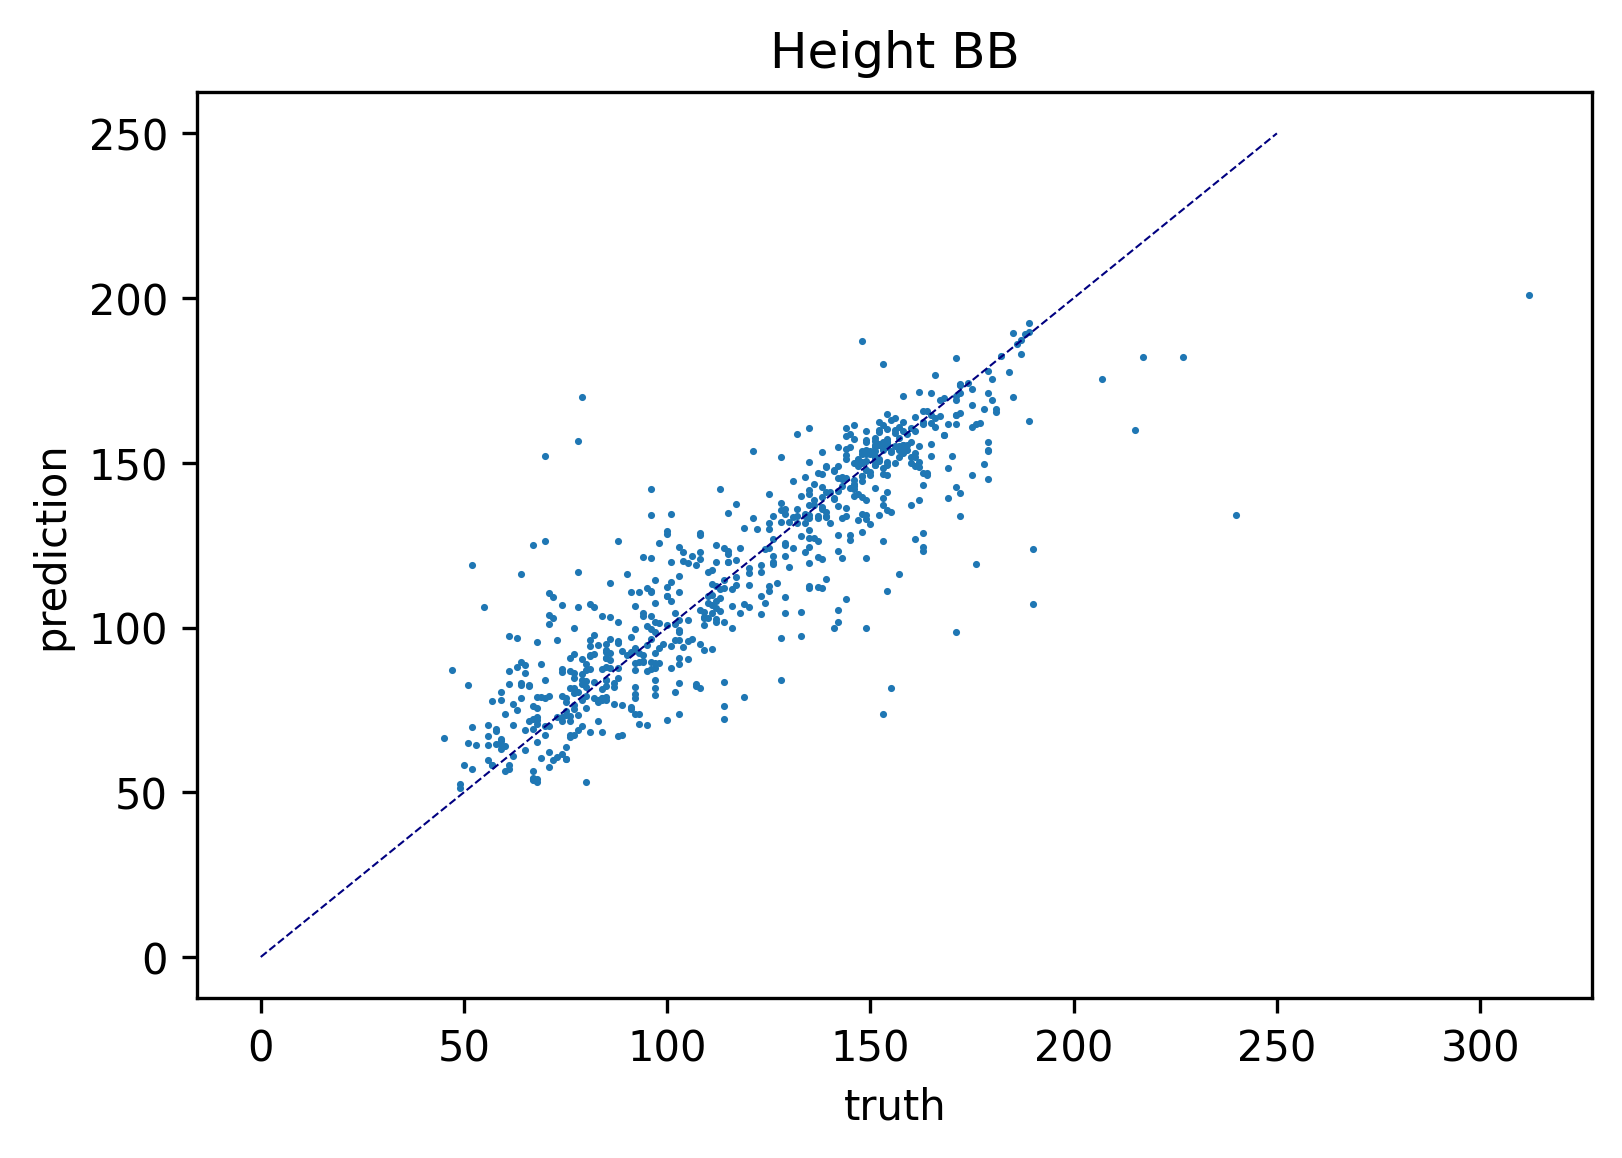
\includegraphics[width=1\textwidth]{bilder/FazitUndAusblick/Grapple_TTAE_Res/Height_BB.png}
 			\subcaption{Rahmenhöhe}			
 		\end{subfigure}
 		\begin{subfigure}[c]{0.49\textwidth}			
 			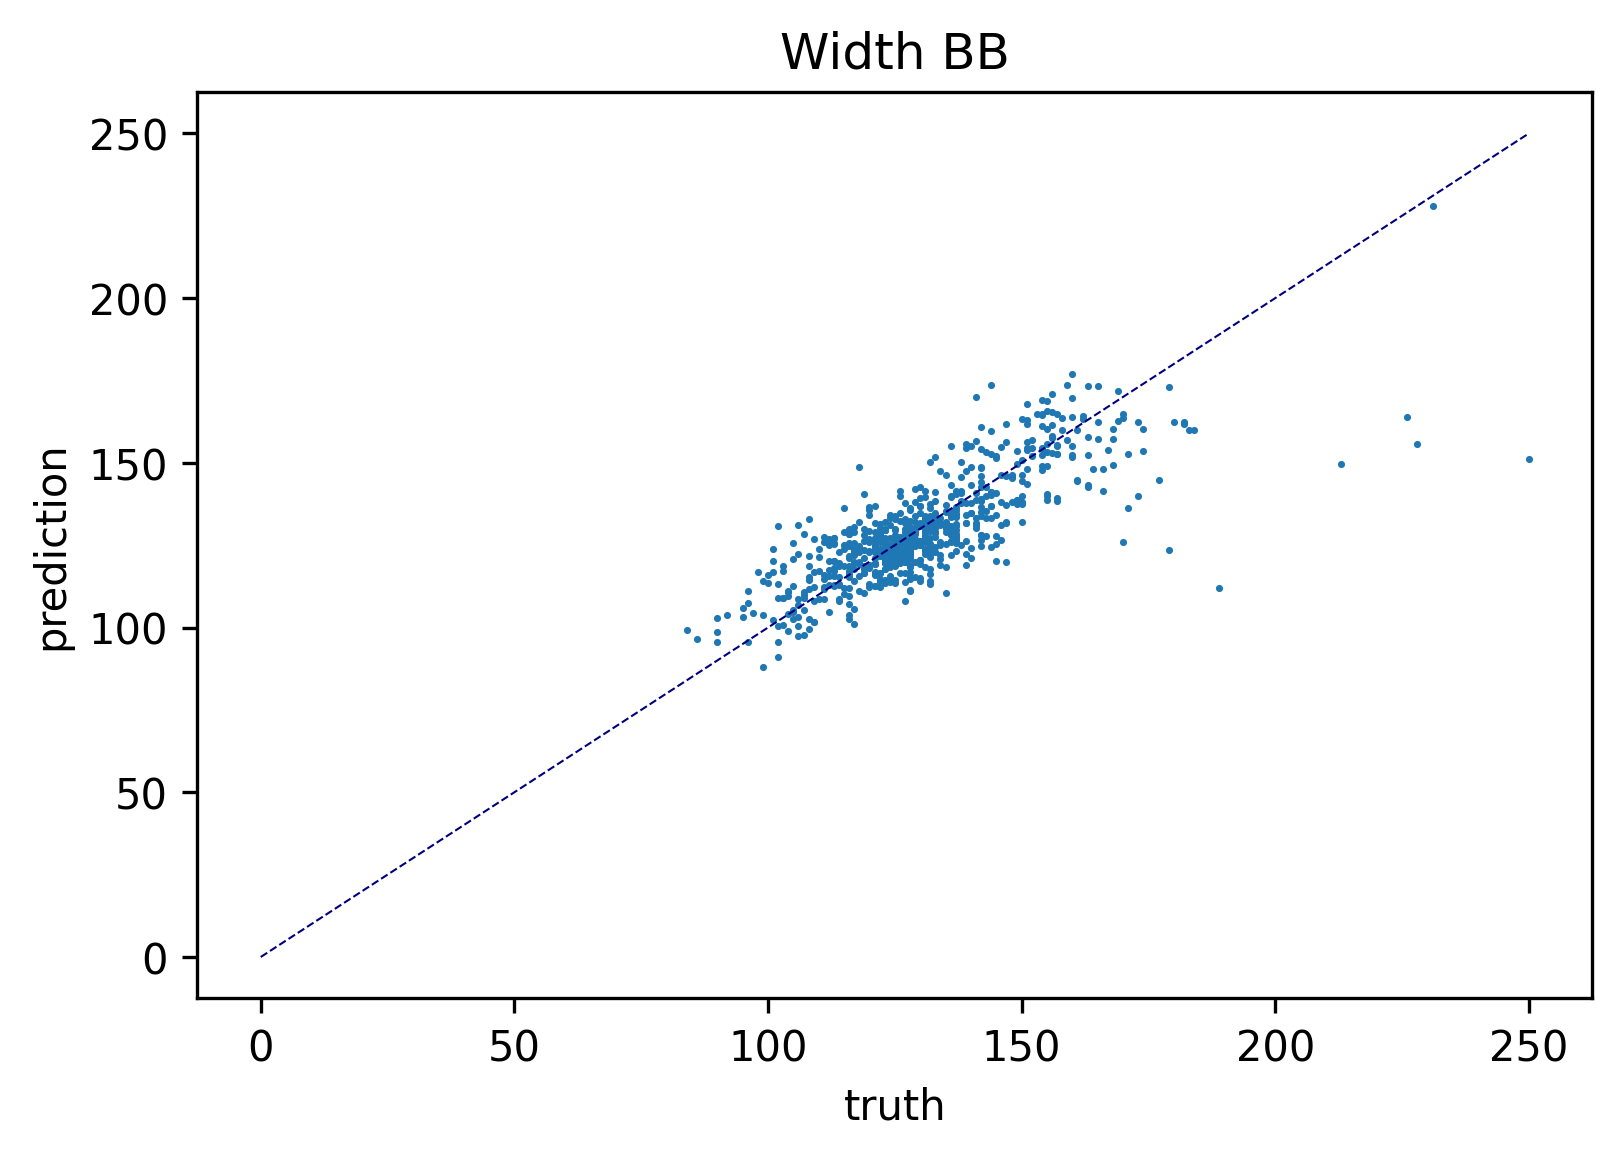
\includegraphics[width=1\textwidth]{bilder/FazitUndAusblick/Grapple_TTAE_Res/Width_BB.png}
 			\subcaption{Rahmenbreite}			
 		\end{subfigure}  
 		\caption{Beschriftung vs Vorhersage}
 		\label{img:TTGrappleLabelVsPred}
 	\end{figure}
 
 	\begin{figure}[h]
 		\centering
 		\begin{subfigure}[c]{0.45\textwidth}			
 			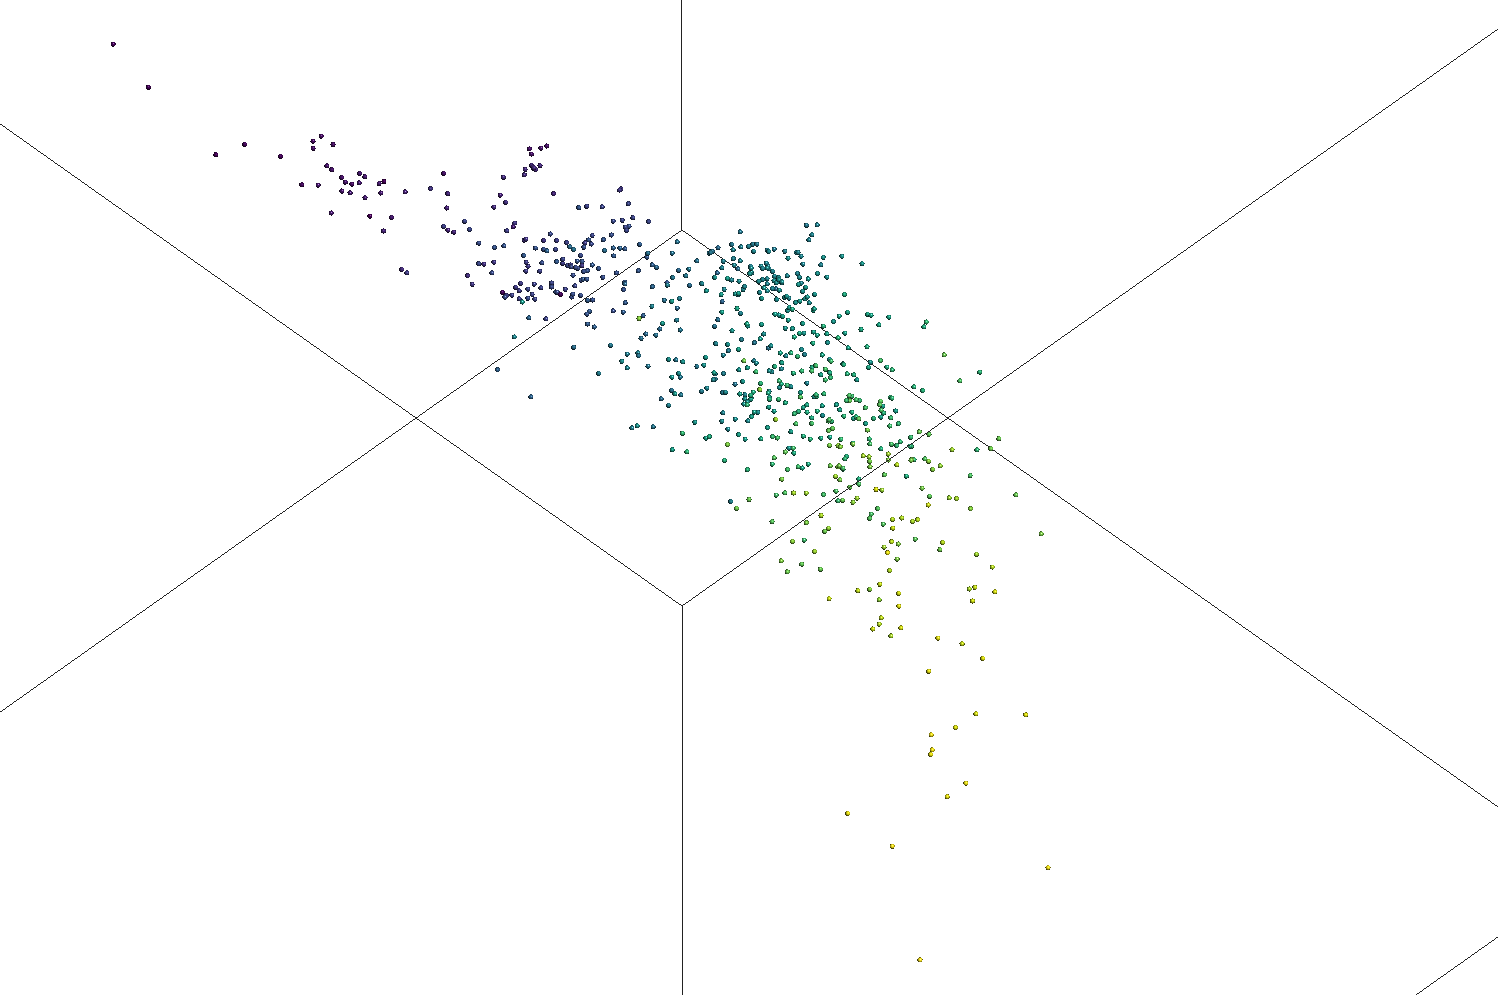
\includegraphics[width=1\textwidth]{bilder/FazitUndAusblick/Grapple_TTAE_Res/TT_Emb_y.png}
 			\subcaption{Einbettung mit y-Position des Greifers - hell nach dunkel entspricht Greiferposition von hoch nach tief}			
 		\end{subfigure}
 		\begin{subfigure}[c]{0.45\textwidth}			
 			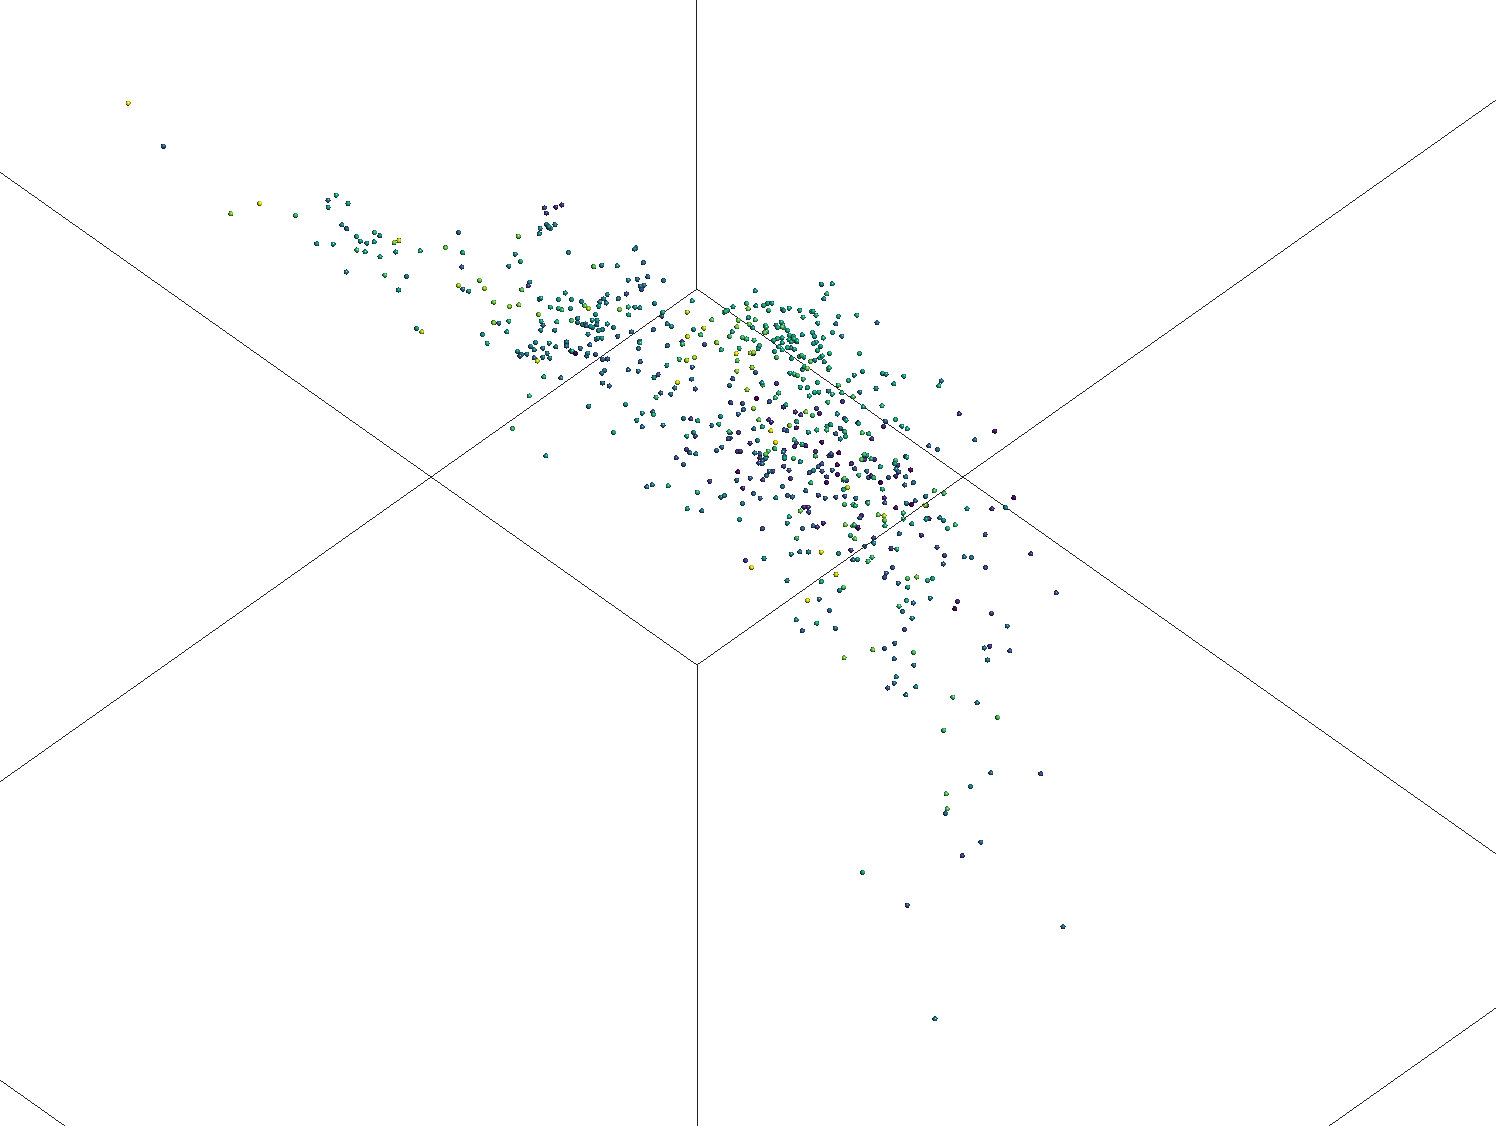
\includegraphics[width=1\textwidth]{bilder/FazitUndAusblick/Grapple_TTAE_Res/TT_Emb_x.png}
 			\subcaption{Einbettung mit x-Position des Greifers - hell nach dunkel entspricht Greifer von Breitseite zu Schmalseite}			
 		\end{subfigure}
 		\begin{subfigure}[c]{0.6\textwidth}			
 			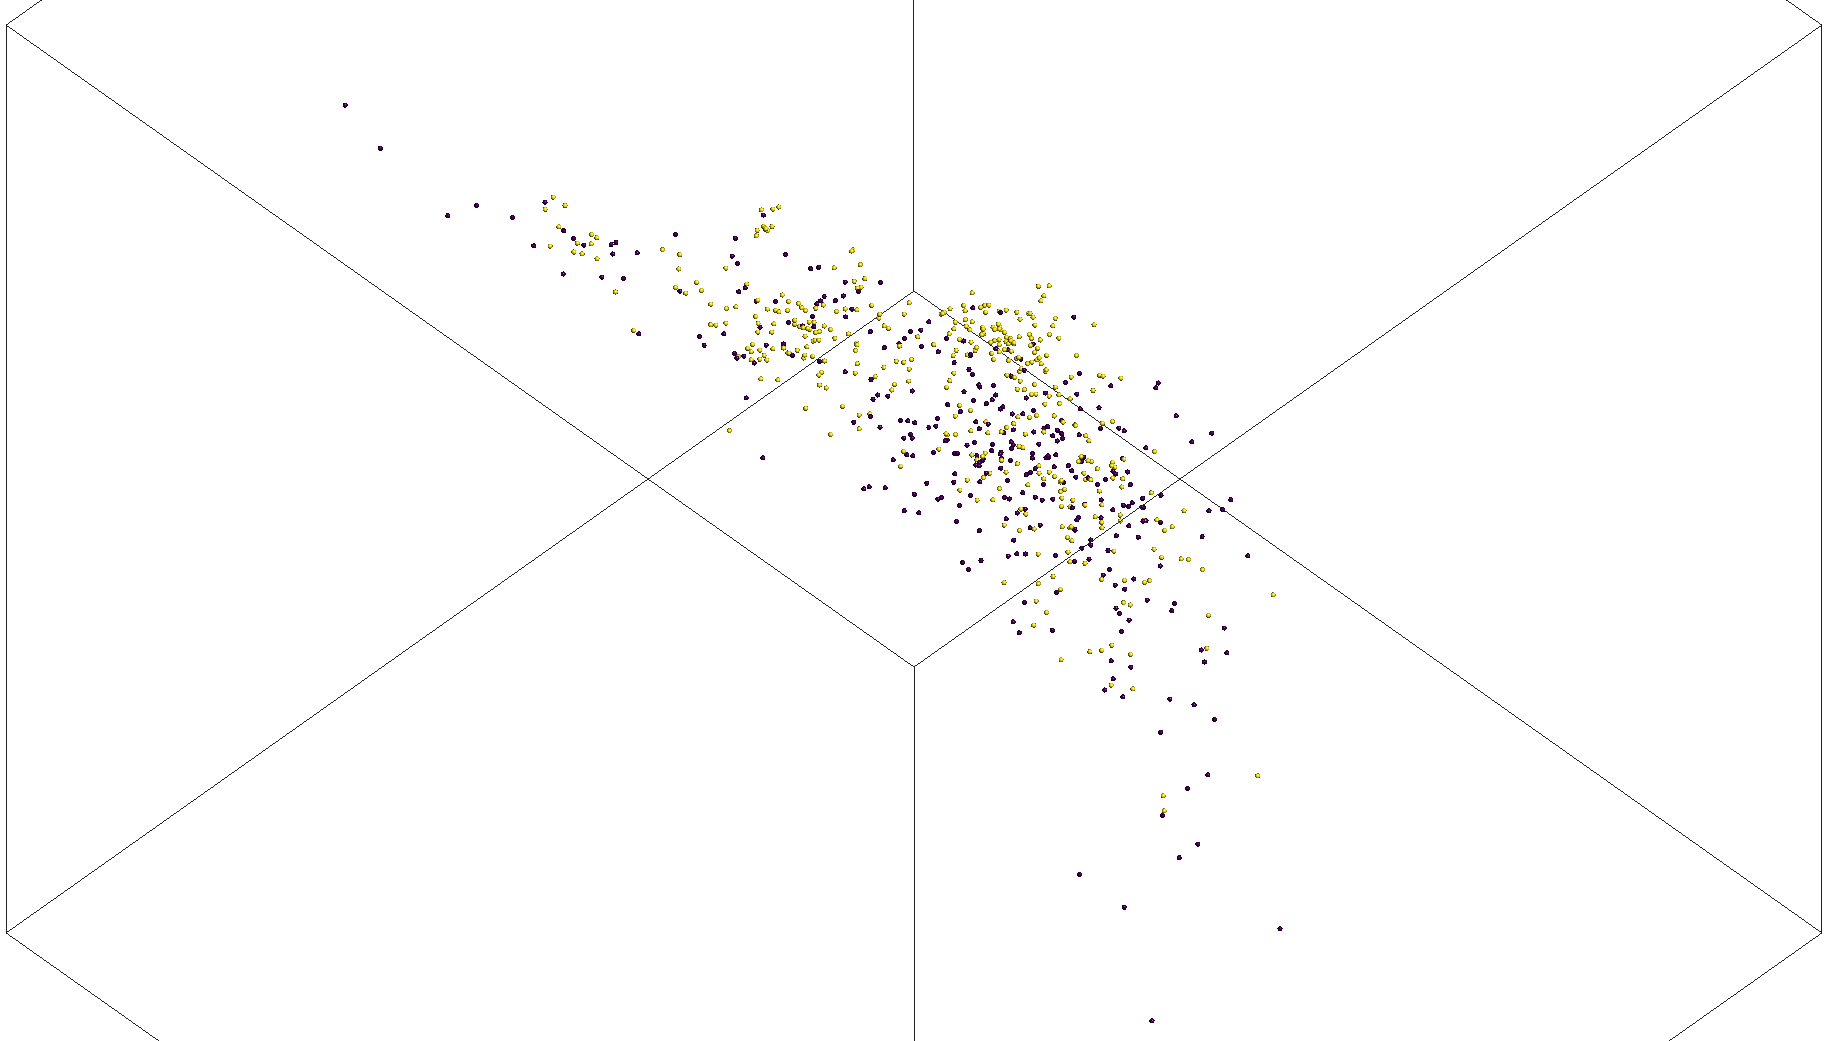
\includegraphics[width=1\textwidth]{bilder/FazitUndAusblick/Grapple_TTAE_Res/TT_Emb_pred.png}
 			\subcaption{Einbettung mit Vorhersage}		
 			\label{img:TTGrappleEinbettungVorhersage}	
 		\end{subfigure}
 		\caption{Einbettung TTAE-Greifererkennung}
 		\label{img:TTGrappleEmb}
 	\end{figure}
 	
	\subsection{Autocrane-Datensatz}
	\label{subsec:AutocraneDatensatz}	
	Im Rahmen der Arbeit wurde ein Datensatz erarbeitet und Projektpartnern zur Verfügung gestellt. Eine spätere Veröffentlichung des Datensatzes unter der Adresse psiori.com ist geplant. Der Datensatz soll zu allgemeinen akademischen und pädagogischen Zwecken genutzt werden dürfen. Alternativ kann Zugang zu dem Datensatz über die E-Mail-Adresse info@psiori.com angefragt werden.

	\subsection{Erweiterung: Multi-Task-Learning-Ansatz}
	\label{subsec:MehrfacheAufgaben}
	\acl{mtl} beschränkt sich nicht auf zwei Aufgaben. Die gezeigte Lösung kann um weitere Aufgaben erweitert werden. In Abbildung \ref{img:AusblickMultiTaskAnsatz} ist der erweiterte Ansatz schematisch abgebildet. Wie in den bisherigen Ansätzen werden ausgehend von der Code-Schicht weitere Aufgaben bearbeitet. Durch die weiteren Aufgaben wird die Gewichtung der einzelnen Aufgaben noch schwerer. In Experiment \ref{subsec:AutoMLExperiment}  wurde gezeigt, dass AutoML bei der Gewichtung helfen kann. Dieser erweiterte Ansatz soll in einem Anschlussprojekt für die Praxistauglichkeit untersucht werden. Der Aufwand, das bisher entwickelte Python-Modul zu erweitern, wird sich dabei in Grenzen halten. Insbesondere müssen im Konstruktor Erweiterungen zum Erstellen der Modelle der weiteren Aufgaben getätigt werden. An anderen Stellen wie z. B. der Methode zum Trainieren des Gesamtmodells wird keine Erweiterung notwendig sein, da bereits mit Listen gearbeitet wird.
	\begin{figure}[h]
		\centering
		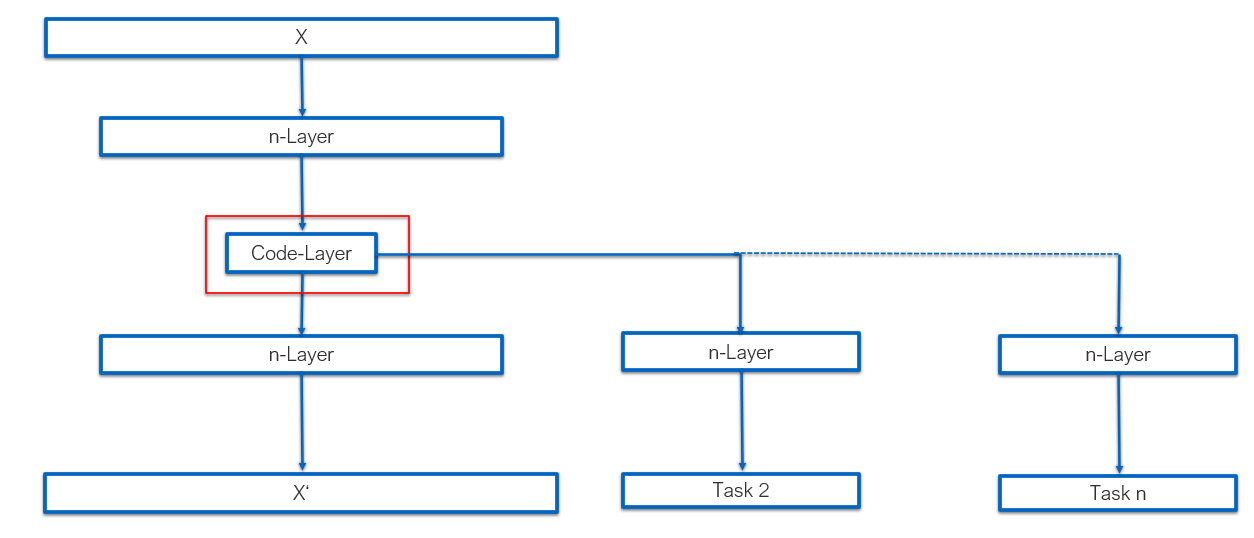
\includegraphics[width=0.6\textwidth, center]{bilder/FazitUndAusblick/MultiTaskAnsatz.PNG}
		\caption{Multi-Task-Learning-Ansatz}
		\label{img:AusblickMultiTaskAnsatz}
	\end{figure}

	\subsection{Flexibilität der Werkzeuge}
	\label{subsec:FlexibilitätDerWerkzeuge}
	Die bisherigen Module sind starr bei der Anwendung. Es ist notwendig, ein \acl{mtl}-Modell zu erstellen, um anschließend den modellbasierten Transfer durchzuführen. Soll ein neuer modellbasierter Transfer durchgeführt werden, ist es zwingend erforderlich, dass dies vom \acl{mtl}-Modell ausgeht. Es ist nicht möglich ein Transfermodell aus einem anderen Transfermodell zu erzeugen. Als mögliche Erweiterung der Module empfiehlt sich, eine Flexibilisierung des Gesamtansatzes durchzuführen. Durch eine Anpassung bei der Modellerstellung der Module ist die Abfolge nicht mehr notwendig. Es ist vorstellbar, dass ein neues Modell, basierend von einer Architekturdefinition komplett neu trainiert wird, oder, ausgehend von einem Autoencoder-Modell, mit beliebig vielen weiteren Aufgaben trainiert werden kann. Konkret muss im Konstruktor der Module eine Zusammenführung der bisher getrennten Ansätze durchgeführt werden.     


	   